\documentclass[MASTER.tex]{subfiles}
\begin{document}

%
%This page uses the following packages. Make sure that you can load them before trying to run the examples on this page. 
%If you do not have a package installed, run: install.packages("packagename"), or if you see the version is out of date, run: update.packages().
 
\begin{frame}
	%R Data Analysis Examples: Poisson Regression
	
	{\Large
		Poisson Regression
	}
	\begin{itemize}
		\item Poisson regression is used to model count variables.
		\item Poisson regression has a number of extensions useful for count models.

	\end{itemize}
\end{frame}




%require(ggplot2)
%require(sandwich)
%require(msm)
% 
%Version info: Code for this page was tested in R version 3.1.1 (2014-07-10)
% On: 2014-08-11
% With: sandwich 2.3-1; boot 1.3-11; knitr 1.6; pscl 1.04.4; vcd 1.3-1; gam 1.09.1; coda 0.16-1; mvtnorm 1.0-0; GGally 0.4.7; plyr 1.8.1; MASS 7.3-33; Hmisc 3.14-4; Formula 1.1-2; survival 2.37-7; psych 1.4.5; reshape2 1.4; msm 1.4; phia 0.1-5; RColorBrewer 1.0-5; effects 3.0-0; colorspace 1.2-4; lattice 0.20-29; pequod 0.0-3; car 2.0-20; ggplot2 1.0.0
%\end{frame}

%%================================================================================================%
%\begin{frame}[fragile]
%
%\frametitle{Poisson Regression with \texttt{R}}
%\Large 
%Please note: The purpose of this page is to show how to use various data analysis commands. It does not cover all aspects of the research process which researchers are expected to do. In particular, it does not cover data cleaning and checking, verification of assumptions, model diagnostics or potential follow-up analyses.
%\end{frame}

 %================================================================================================%
\begin{frame}[fragile]

\frametitle{Poisson Regression with \texttt{R} } 
 
 \Large	
 
 \textbf{Examples of Poisson regression} \\
 	
 \begin{itemize}	
 \item The number of awards earned by students at a secondary or high school. 
 \item Predictors of the number of awards earned include the type of program in which the student was enrolled (e.g., vocational, general or academic) and the score on their final exam in math.
 \end{itemize}
 
\end{frame}

%================================================================================================%
\begin{frame}[fragile]
	
	\frametitle{Poisson Regression with \texttt{R}}
	\Large
	\textbf{Conventional OLS regression}
	\begin{itemize}
		\item Count outcome variables are sometimes log-transformed and analyzed using OLS regression. 
		\item Many issues arise with this approach, including loss of data due to undefined values generated by taking the log of zero (which is undefined) and biased estimates.
	\end{itemize}
	\bigskip
\end{frame}


%================================================================================================%
\begin{frame}[fragile]

\frametitle{Poisson Regression with \texttt{R}}
\Large
\textbf{Description of the data}

\begin{itemize}
\item For the purpose of illustration, we have simulated a data set for the last example.

\item The data set is called \textit{poissonreg.csv}  

\item In this example, \textbf{num\_awards} is the outcome variable and indicates the number of awards earned by students at a high school in a year

\end{itemize}
\end{frame}
%================================================================================================%
\begin{frame}[fragile]
	
	\frametitle{Poisson Regression with \texttt{R}}
	\Large
	\textbf{Predictor Variables}
\begin{itemize}
\item \textbf{math} is a continuous predictor variable and represents students' scores on their math final exam, \item \textbf{prog} is a categorical predictor variable with three levels indicating the type of program in which the students were enrolled.

\item  \textbf{prog} is coded as 1 = "\textit{General}",
 2 = "\textit{Academic}" and 3 = "\textit{Vocational}". 
\end{itemize}
% Let's start with loading the data and looking at some descriptive statistics.

\end{frame}

%%================================================================================================%
%\begin{frame}[fragile]
%
%\frametitle{Poisson Regression with \texttt{R}}
%\Large
%
%\begin{verbatim}
%p <- read.csv("http://www.ats.ucla.edu/stat/data/poisson_sim.csv")
%p <- within(p, {
%  prog <- factor(prog, levels=1:3, labels=c("General", "Academic", "Vocational"))
%  id <- factor(id)
%})
%summary(p)
%\end{verbatim}
%\end{frame}

%================================================================================================%
\begin{frame}[fragile]
	
\frametitle{Poisson Regression with \texttt{R}}
\normalsize
	\begin{verbatim}
        id        num_awards           prog          math     
1      :  1   Min.   :0.00   General   : 45   Min.   :33.0  
2      :  1   1st Qu.:0.00   Academic  :105   1st Qu.:45.0  
3      :  1   Median :0.00   Vocational: 50   Median :52.0  
4      :  1   Mean   :0.63                    Mean   :52.6  
5      :  1   3rd Qu.:1.00                    3rd Qu.:59.0  
6      :  1   Max.   :6.00                    Max.   :75.0  
  (Other):194
\end{verbatim}
\end{frame}
%================================================== %	
\begin{frame}
	\begin{figure}
		\centering
		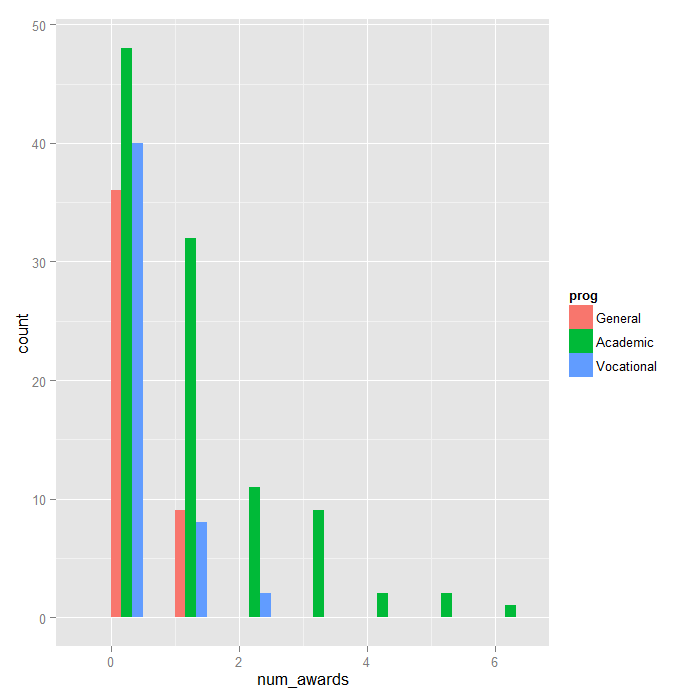
\includegraphics[width=0.8\linewidth]{poisson1}
		\caption{}
		\label{fig:poisson1}
	\end{figure}
	
	
\end{frame}
%================================================================================================%
\begin{frame}[fragile]

\frametitle{Poisson Regression with \texttt{R}}
\Large

\begin{itemize}
\item Each variable has 200 valid observations and their distributions seem quite reasonable. 
\item The mean and variance of our outcome variable are more or less the same. 
\item Our model assumes that these values, conditioned on the predictor variables, will be equal (or at least roughly so).
\end{itemize}
\end{frame}
%================================================================================================%
%\begin{frame}[fragile]
%\frametitle{Poisson Regression with \texttt{R}}
%We can use the tapply function to display the summary statistics by program type. The table below shows the average numbers of awards by program type and seems to suggest that program type is a good candidate for predicting the number of awards, our outcome variable, because the mean value of the outcome appears to vary by prog.
%\end{frame}
%\end{document}
%================================================================================================%
\begin{frame}[fragile]
\frametitle{Poisson Regression with \texttt{R}}
\Large
\begin{itemize}
\item Additionally, the means and variances within each level of prog--\textit{the conditional means and variances}--are similar. 
\item A conditional histogram separated out by program type is plotted to show the distribution.
\end{itemize}


\end{frame}

%%================================================================================================%
%\begin{frame}[fragile]
%
%\frametitle{Poisson Regression with \texttt{R}}
%\Large
%
%\begin{verbatim}
%
%ggplot(p, aes(num_awards, fill = prog)) +
%  geom_histogram(binwidth=.5, position="dodge")
%
%\end{verbatim}
%
% \end{frame}
%================================================================================================%
		
%with(p, tapply(num_awards, prog, function(x) {
%	sprintf("M (SD) = %1.2f (%1.2f)", mean(x), sd(x))
%}))
%
%General               Academic             Vocational 
%"M (SD) = 0.20 (0.40)" "M (SD) = 1.00 (1.28)" "M (SD) = 0.24 (0.52)"


\end{document}
